\def\CTeXPreproc{Created by ctex v0.2.12, don't edit!}%% ****** Start of file template.aps ****** %
%%
%%
%%   This file is part of the APS files in the REVTeX 4 distribution.
%%   Version 4.0 of REVTeX, August 2001
%%
%%
%%   Copyright (c) 2001 The American Physical Society.
%%
%%   See the REVTeX 4 README file for restrictions and more information.
%%
%
% This is a template for producing manuscripts for use with REVTEX 4.0
% Copy this file to another name and then work on that file.
% That way, you always have this original template file to use.
%
% Group addresses by affiliation; use superscriptaddress for long
% author lists, or if there are many overlapping affiliations.
% For Phys. Rev. appearance, change preprint to twocolumn.
% Choose pra, prb, prc, prd, pre, prl, prstab, or rmp for journal
%  Add 'draft' option to mark overfull boxes with black boxes
%  Add 'showpacs' option to make PACS codes appear
%  Add 'showkeys' option to make keywords appear
\documentclass[pra,preprint,superscriptaddress,showkeys,showpacs]{revtex4}
%\documentclass[aps,prl,preprint,superscriptaddress]{revtex4}
%\documentclass[aps,prl,twocolumn,groupedaddress]{revtex4}

% You should use BibTeX and apsrev.bst for references
% Choosing a journal automatically selects the correct APS
% BibTeX style file (bst file), so only uncomment the line
% below if necessary.
\bibliographystyle{apsrev}
\usepackage{amsmath}
\usepackage{graphicx}
\begin{document}

% Use the \preprint command to place your local institutional report
% number in the upper righthand corner of the title page in preprint mode.
% Multiple \preprint commands are allowed.
% Use the 'preprintnumbers' class option to override journal defaults
% to display numbers if necessary
%\preprint{}

%Title of paper
\title{ Thermal rectification in coupled rotor lattices with gradient mass}

% repeat the \author .. \affiliation  etc. as needed
% \email, \thanks, \homepage, \altaffiliation all apply to the current
% author. Explanatory text should go in the []'s, actual e-mail
% address or url should go in the {}'s for \email and \homepage.
% Please use the appropriate macro for each each type of information

% \affiliation command applies to all authors since the last
% \affiliation command. The \affiliation command should follow the
% other information
% \affiliation can be followed by \email, \homepage, \thanks as well.
\author{M. An}
\author{J. N. Zhou}
\author{F. G. Li}
\author{J. W. Xiong}

%\homepage[]{}a

%\thanks{}
%\altaffiliation{}
\affiliation{ School of Physics and Telecommunication
Engineering, South China Normal University, 510006 Guangzhou, China}

%Collaboration name if desired (requires use of superscriptaddress
%option in \documentclass). \noaffiliation is required (may also be
%used with the \author command).
%\collaboration can be followed by \email, \homepage, \thanks as well.
%\collaboration{}
%\noaffiliation

%\date{\today}
\begin{abstract}
\indent Heat conduction through one-dimensional (1D) coupled rotator
lattices is investigated in the presence of mass gradient. It is found that thermal current in the
direction of mass increasing is not asymmetric with heat flux though
mass decreasing system, which is called thermal rectification.
Moreover, we find that the larger is the mass gradient, the more
evident is the thermal rectification effect, which is consistent
with FPU lattice with mass gradient. Based on the influences
of the thermal rectification on shape parameters $K$ and $A$ of
nearest-neighbor interactions, the average temperature of atomic
chain and the system size, a optimum thermal rectifier is designed,
which thermal rectification efficiency has reached 70. These
investigations would contribute to controlling and manipulating
thermal current.
\end{abstract}

% insert suggested PACS numbers in braces on next line
\pacs{05. 40. Fb, 02. 50. Ey, 05. 40. -a}
% insert suggested keywords - APS authors don't need to do this
\keywords{Heat conduction, coupled rotor lattices,thermal rectification }

%\maketitle must follow title, authors, abstract, \pacs, and \keywords

% body of paper here - Use proper section commands
% References should be done using the \cite, \ref, and \label commands


%\maketitle must follow title, authors, abstract, \pacs, and \keywords
\maketitle
\section {Introduction}
\indent Heat conduction is an ancient physical question, which was
described by Fourier Law as $J=\kappa{\Delta T}$ where $\kappa$ is a
constant, independent of system size. However, in recent years
plenty of investigations have suggested that heat conduction in low
dimensional systems diverges as the system size, for example
FPU-$\alpha$, FPU-$\beta$, diatomic $Toda$ and so on\cite{a1}. These
discoveries have attracted massive attention on heat conduction in
low dimensional systems. Especially, the proposal\cite{a2} of
processing information by controlling and manipulating phonons(heat
carrier) has motivated people to have designed various thermal
devices, similar to electronic counterparts, thermal
transistors\cite{a3}, thermal logic gates\cite{a4}, thermal
memory\cite{a5} and thermal limiters\cite{a6}. To our delighted, the
solid state thermal rectifier from carbon nanotubes(CNTS) with
nonuniform axial mass distribution has been realized
experimentally\cite{a7}.\\
\indent There exists various studies of designing various thermal
rectifiers and negative differential thermal resistance \cite{a8,a9,a10,a11,a12,a13,a14,a15,a16,a17,a18,a19,a20,a21,a22,a23,a24,a25}.
 Li and his-coworker firstly presented the model\cite{a8} consisting of three segment FK
chain of different interaction parameters to control the strength of
the substrate potential. Later on, another models\cite{a9,a10}
coupled two nonlinear one dimensional lattices increase the thermal
rectification magnitude greatly. These investigations have been
explained by mismatch/match of frequency spectrum at the two ends of
the chain. Yang and his-coworker\cite{a19} theoretically showed
thermal rectification in graded mass of FPU-$\beta$ lattices, and
found that the larger is the mass gradient, the more obvious is the
thermal rectification effect. Subsequently, Shah\cite{a20} studied
the FPU-$\beta$ lattices with exponential mass graded lattices, and
showed that the exponential mass graded material is a better and
genuine choice for thermal rectification. Hu\cite{a21} explored the
thermal rectifiacion in one dimensional mass-graded harmonic lattice
with harmonic and anharmonic on-site potential. It was found that
thermal rectification occurs in the model with the anharmonic
on-site potential and vanishes with the harmonic one, which suggests
nonlinearity is necessary for thermal rectification. On the other
hand, extensive investigations have done to determine the mechanisms
that lead to thermal rectification in graded mass systems. Nan and
Wang found that thermal rectification results from the transmission
of high-frequency phonons by applying the nonequilibrium Green's
function method\cite{a24}. Emmanuel have showed the graded
anharmonic systems as genuine thermal
rectifier by applying self-consistent reservoirs\cite{a22}. Zhong and co-workers \cite{a25} found that graphene nanoribbons with thickness-asymmetry have a good thermal rectification and the thermal rectification factor depends on temperature as well as the thickness-ratio of the
two-segment.\\
\indent In this paper, we investigate one-dimensional (1D) graded
mass lattices with nonlinear nearest-neighbor interactions, and
discover thermal rectification. In order to amplify the thermal
rectification effect, the dependence of thermal rectification on the
mass gradient, the shape parameter $A$ and $K$, the average
temperature $T_{0}$ and the system size have been investigated.
\section{Model and Methods}
\indent  The Hamilton of one-dimensional (1D) chain under
consideration is of the form \cite{a1,a2}
\begin{equation}\label{}
    H=\sum^{N}_{i=1}\frac{P^{2}_{i}}{2M_{i}}+V(x_{i+1}-x_{i})+U(x_{i}),
\end{equation}
where $x_{i}$ is the instantaneous displacement of the $ith$
particle from its equilibrium position, $P_{i}$ denotes the $ith$
particle's instantaneous momentum, $M_{i}$ is the $ith$ mass of the
particle. $V(x_{i+1}-x_{i})$ is the nearest-neighbor interaction
potential, $U(x_{i})$ is the on-site potential. $N$ is the total
number of particles in the chain. In the coupled rotator model $V$
takes an anharmonic form \cite{a1,a2}
\begin{equation}\label{}
V=K(1-\cos A(x_{i}-x_{i-1})), U(x_{i})=0.
\end{equation}
For linear mass gradient, the mass of the $ith$ particle is given by
 $M_{i}=M_{max}-(i-1)(M_{max}-M_{min})/(N-1)$, where $M_{max}$ is the  mass of
 the particle at left end (first particle) and $M_{min}$ is the mass of the particle
 at right end (last particle) of the chain. In our simulation, Langevin heat baths\cite{a1} were imposed on the two ends
 and the fixed-boundary conditions $x_{0}=x_{N+1}=0$ were adopted.
Therefore the equations of motion are:
\begin{equation}\label{}
M_{i}\ddot{x}_{i}=-\frac{\partial{H}}{\partial{x_{i}}}-\gamma_{i}\dot{x}_{i}+\eta_{i},
\end{equation}
where $\gamma_{i}=\gamma(\delta_{i,1}+\delta_{i,N})$ and
$\eta_{i}=\eta_{H}\delta_{i,1}+\eta_{L}\delta_{i,N}$. The equations
of motion for the central particles $(i=2,3...,N-1)$ are,
\begin{equation}\label{}
M_{i}\ddot{x}_{i}=KA[\sin{A(x_{i+1}-x_{i})}-\sin{A(x_{i}-x_{i-1})}],
\end{equation}
the equations of motion for $i=1$ and $i=N$ particles are given by,
\begin{equation}\label{}
\begin{aligned}
M_{1}\ddot{x}_{1}=&KA[\sin{A(x_{2}-x_{1})}-\sin{A(x_{1}-x_{0})}]-\gamma{\dot{x}_{1}}\\
&+\eta_{H}(t),
\end{aligned}
\end{equation}
\begin{equation}
\begin{aligned}\label{}
M_{N}\ddot{x}_{N}=&KA[\sin{A(x_{N+1}-x_{N})}-\sin{A(x_{N}-x_{N-1})}]\\
&-\gamma{\dot{x}_{N}}+\eta_{L}(t),
\end{aligned}
\end{equation}
where $\gamma$ is the friction coefficient. The dot stands for the
derivation with respect to time $t$. The noise terms $\eta_{\pm}(t)$
denote a Gaussian white noise that satisfies the fluctuation
dissipation relations
\begin{equation}
\langle\eta_{H}(t)\eta_{H}(t^{'})\rangle=2\gamma{k_{B}}T_{H}\delta{(t-t^{'})},
\end{equation}
\begin{equation}
\langle\eta_{L}(t)\eta_{L}(t^{'})\rangle=2\gamma{k_{B}}T_{L}\delta{(t-t^{'})},
\end{equation}
$k_{B}$ denotes Boltzmann's constant and we set $k_{B}$=1 and
$\gamma=1$ in our
simulations. \\
\indent In this paper, we set $T_{H}=T_{0}(1+\Delta T)$ and
$T_{L}=T_{0}(1-\Delta T)$, where $T_{0}=(T_{H}+T_{L})/2$ is the
average temperature and $\Delta T=T_{H}-T_{L}$ is the temperature
bias of the two ends
 of particle chain. We set $J_{L}$ as the thermal current in the direction of mass decreasing when the
 high temperature bath (on the left) was imposed on $M_{max}$ (the maximum particle mass), and $J_{R}$ as the
 heat flux in the direction of mass increasing when the high temperature bath (on the right) was coupled
 with $M_{min}$ (the minimum particle mass).\\
\indent For simplicity, the local heat flux is defined as
$j_{i}=\langle{\dot{x}_{i}}F(x_{i}-x_{i-1})\rangle$, where
F=-$\partial{V}$/$\partial{x}$ and the notation
$\langle{...}\rangle$ denotes a steady-state average. After the
system reaches a stationary state, $j_{i}$ is independent of site
position $i$, so that the local flux can be denoted as $j$ and the
total heat flux $J=Nj$. In our simulations, the equations of
motion(4-6) are integrated by using a second-order stochastic
Runge-Kutta algorithm\cite{a26} with a small time step (h=0.002).
The simulations are performed long enough to allow the system to
reach a nonequilibrium steady state in which the local heat flux is
a constant along the chain.



\section {Numerical results and discussion}
\begin{figure}
\centering
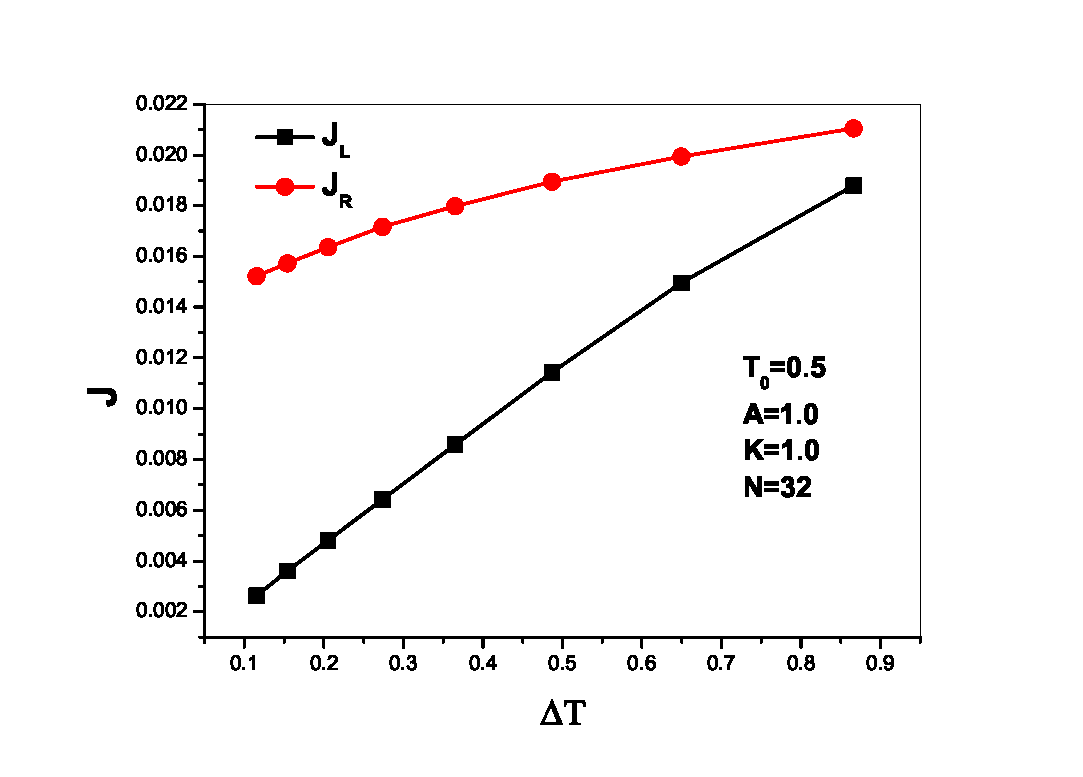
\includegraphics[width=8cm]{fig1.eps}
\caption{The  heat flux $J$ as a function of the
temperature gradient $\Delta T$. The parameters are $T_{0}=0.5$,
$A=1.0$, $K=1.0$, $M_{max}=10.0$, $M_{min}=1.0$, $N=32$.}
\end{figure}

\indent Figure 1 presents the dependence of the heat fluxes
($J_{R},J_{L}$) ($J_{L}$ denotes the thermal current from left to
right and $J_{R}$ is the heat flux from right to left) on the
temperature gradient $\Delta T$. It is observed that the heat fluxes
increase as the temperature difference $\Delta T$ increases.
However, compared on $J_{L}$, the amplitude of $J_{R}$ is much
larger, which is called thermal rectification depicting thermal
currents are not asymmetry when the heat baths are reversed.\\
\begin{figure}
\centering
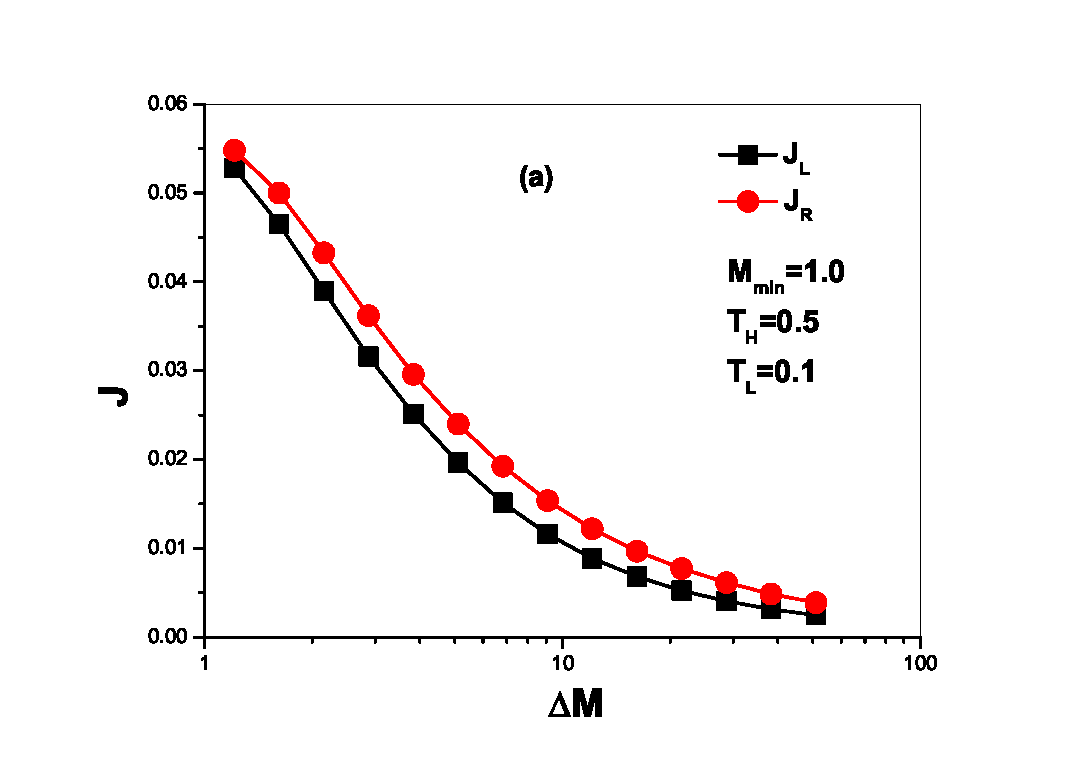
\includegraphics[width=8cm]{fig2a.eps}
\centering
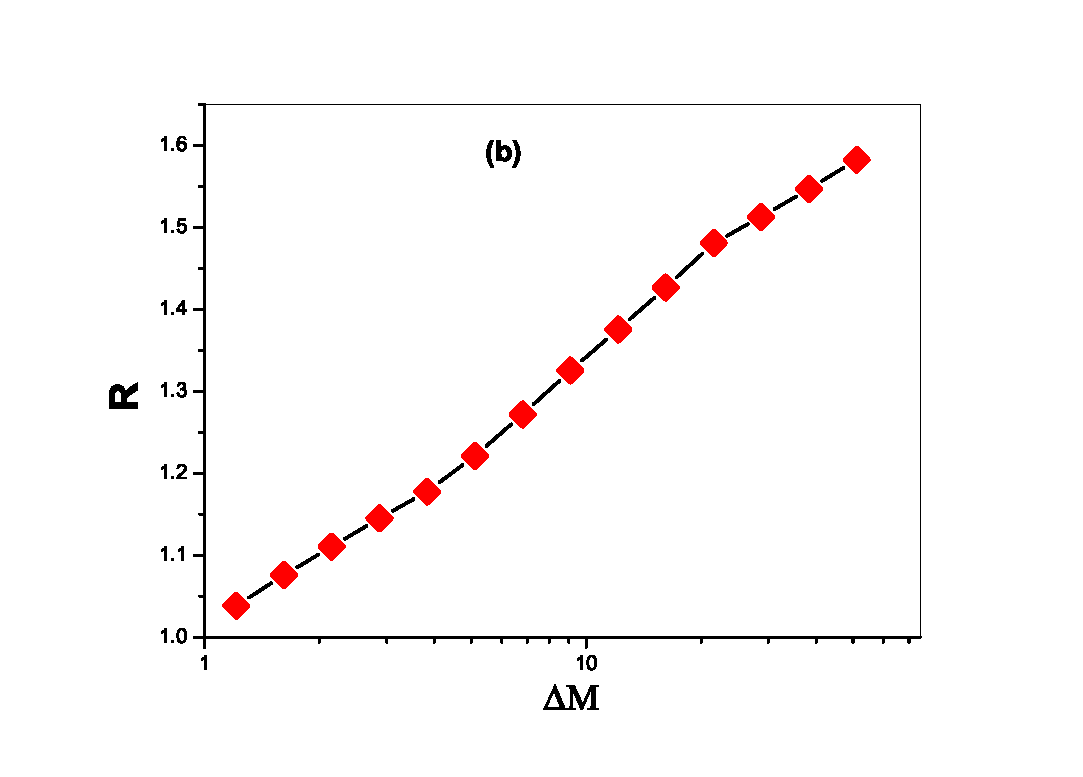
\includegraphics[width=8cm]{fig2b.eps}
\caption{(a)The heat fluxes ($J_{R},J_{L}$) as a function of the mass
gradient $\Delta M$. (b) The dependence of the heat rectification
efficiency $R=\mid J_{R}/J_{L}\mid$ on the mass gradient $\Delta M$.
The parameters are $T_{0}=0.5$, $A=1.0$, $K=1.0$, $M_{min}=1.0$,
$N=32$.}
\end{figure}
\indent Figure 2(a) shows the dependence of the heat fluxes J on the
mass gradient $\Delta M=M_{max}/M_{min}$ at $M_{min}=1.0$ for
$T_{H}=0.5$ and $T_{L}=0.1$. If the mass gradient $\Delta M$ is
increased, heat currents ($J_{R},J_{L}$) through systems decrease
monotonically. Obviously, the heat flux flows more easily in the
direction of mass increasing for any values of mass gradient. It
might be assumed: the uniform distribution of atomic masses and the
nonlinear nearest-neighbor interaction lead to the mismatch of power
spectrum at the two ends of atomic chain. Therefore there exists
asymmetric thermal currents. In order to describe quantitatively the
thermal rectification efficiency, we introduce the ratio $R=\mid
J_{R}/J_{L}\mid$, when $R=1$ shows no thermal rectification effect,
and the larger is
the value of $R=\mid J_{R}/J_{L}\mid$, the better is thermal rectification effect.\\
\indent Figure 2(b) shows the dependence of the rectification
efficiency $R$ on the mass gradient $\Delta M$. As the mass gradient
$\Delta M$ becomes larger, the thermal rectification efficiency R
increases. It is found that the mass gradient $\Delta M$ contributes
to thermal rectification, which is consistent with previous investigations\cite{a19,a20,a21}.\\
\begin{figure}
\centering
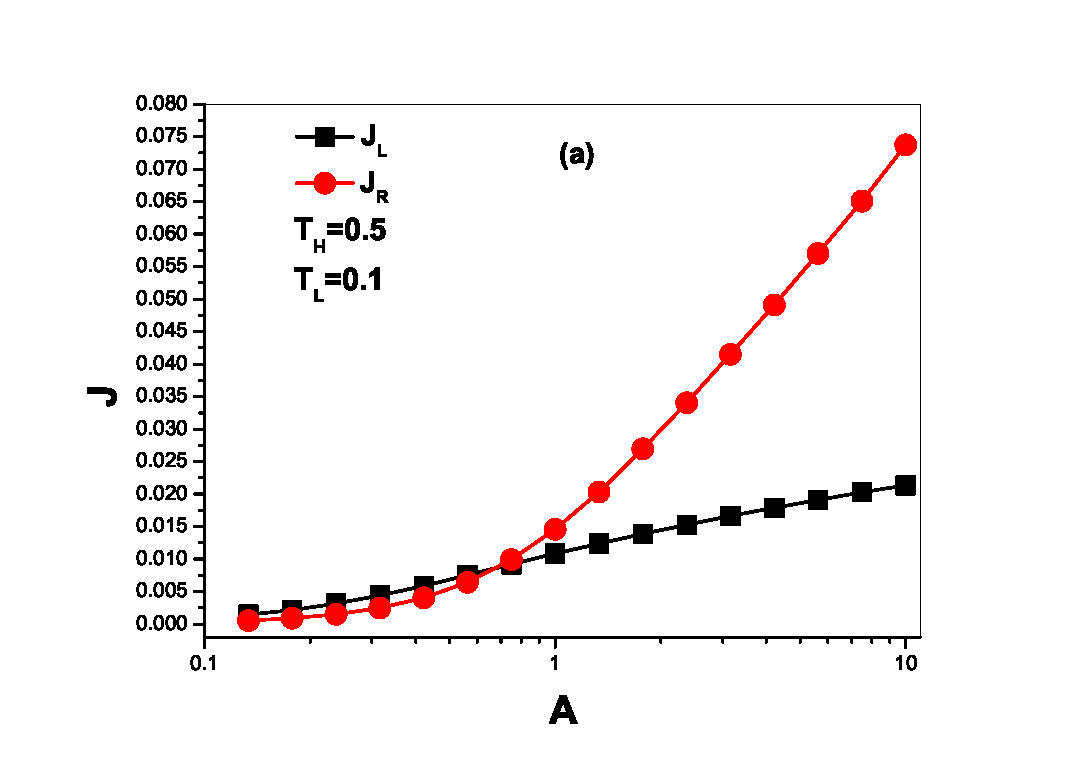
\includegraphics[width=8cm]{fig3a.eps}
\centering
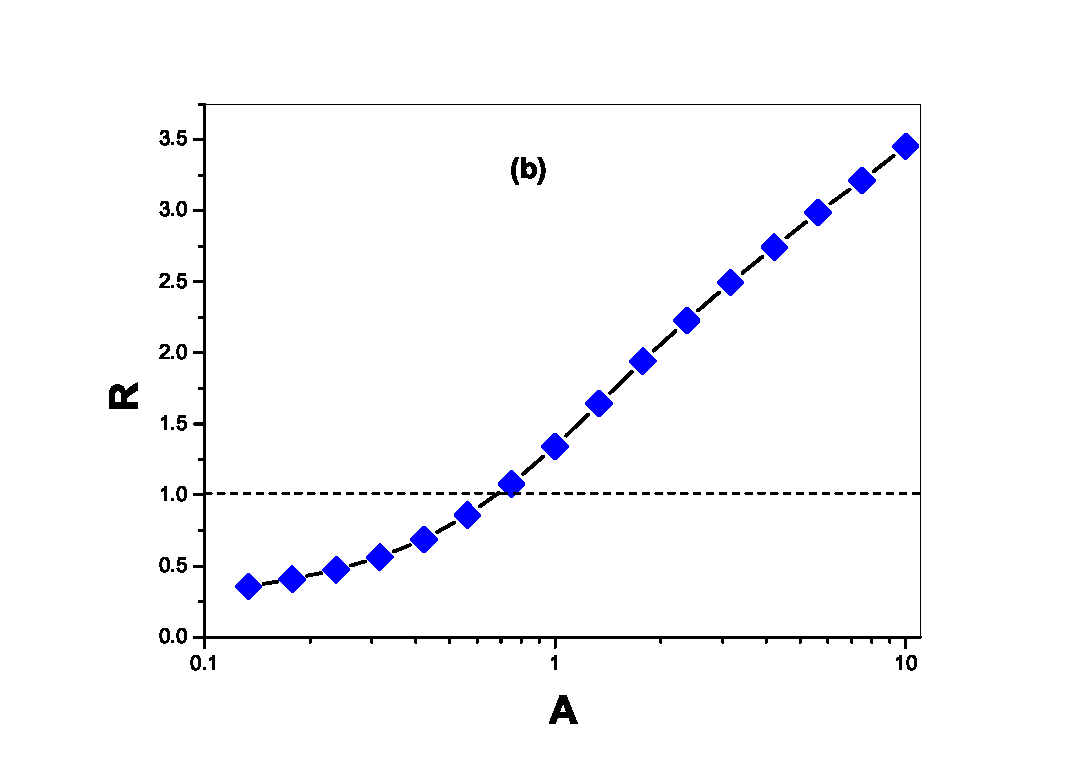
\includegraphics[width=8cm]{fig3b.eps}
\caption{(a) The heat fluxes ($J_{R},J_{L}$) as a function of the
shape parameter $A$ of the nearest-neighbor interaction. (b) the
dependence of the heat rectification efficiency $R=\mid
J_{R}/J_{L}\mid$ on the shape parameter $A$. The parameters are
$T_{L}=0.1$, $T_{H}=0.5$, $K=1.0$, $M_{max}=10.0$, $M_{min}=1.0$,
$N=32$.}
\end{figure}

\indent Figure 3(a) depicts the dependence of the heat currents
($J_{R},J_{L}$) on the shape parameter $A$. The heat fluxes
($J_{R},J_{L}$)all increases with increment of the shape parameter
$A$. It is observed easily that $J_{L}$ and $J_{R}$ do not increase
at the same pace, which suggests the shape parameter $A$ could have
effects on thermal rectification. Because the augment of the shape
parameter $A$ gives rise to a larger nonlinearity of the
nearest-neighbor interaction. It improves the probability of the
umklapp processes, which increases the degree of the mismatch of
power spectrum of the two ends of atomic chain. Based on Figure
3(b), the more evident is the thermal rectification effect,
the larger is the shape parameter $A$ of nearest-neighbor interactions.\\

\begin{figure}
\centering
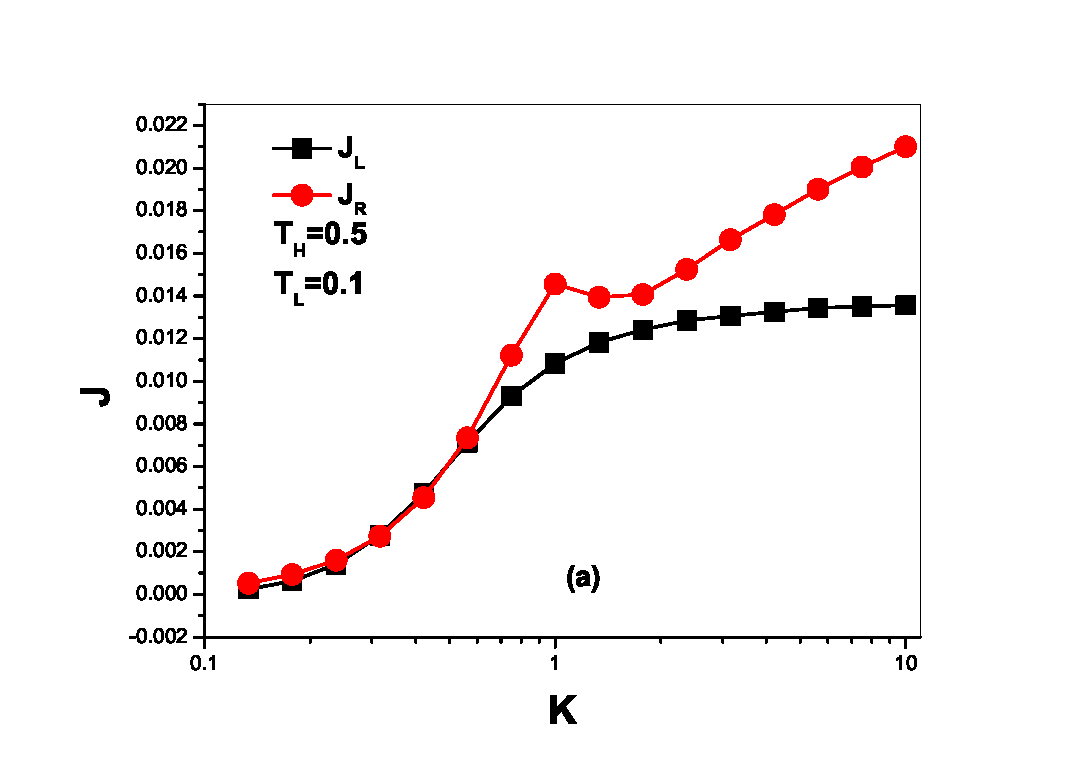
\includegraphics[width=8cm]{fig4a.eps}
\centering
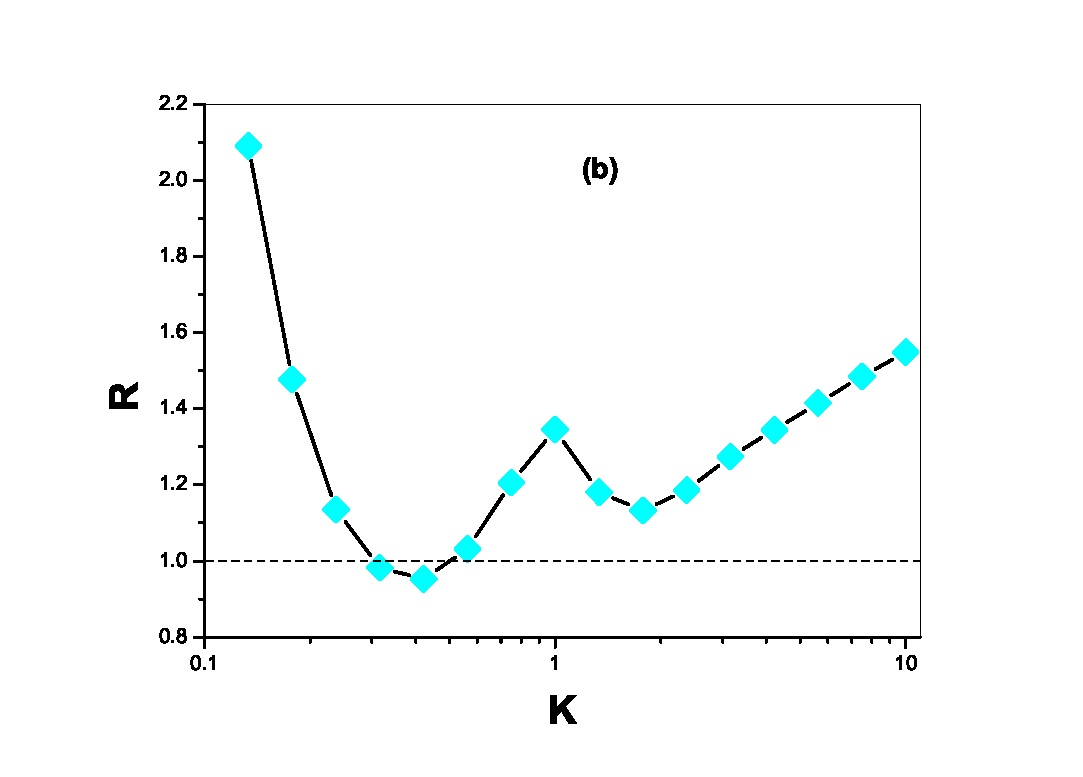
\includegraphics[width=8cm]{fig4b.eps}
\caption{(a)The heat fluxes ($J_{R},J_{L}$) as a function of the
strength $K$ of the nearest-neighbor interaction. (b) the dependence
of the thermal rectification efficiency $R=\mid J_{R}/J_{L}\mid$ on
the strength $K$ of the nearest-neighbor interaction. The parameters
are $T_{L}=0.1$, $T_{H}=0.5$, $A=1.0$, $M_{max}=10.0$,
$M_{min}=1.0$, $N=32$.}
\end{figure}
\indent Figure 4(a) shows the dependence of the heat fluxes $J_{L}$
and $J_{R}$ on the strength $K$ of the nearest-neighbor interaction
at $T_{H}=0.5$ and $T_{L}=0.1$. $J_{L}$ that is the heat flux in the
direction of decreasing mass increases for $K=[0.1, 1.0]$, and
barely changes with increasing the strength $K$ of the
nearest-neighbor interaction. More interestingly, $J_{R}$ that is
the average thermal current in the direction of increasing mass
decreases with the increment of the strength $K$ of the
nearest-neighbor interaction (further investigations see Fig. 5).
Figure 4(b) describes that the thermal rectification ratio $R$ as a
function of the strength $K$ of the nearest-neighbor interaction. It
is found that the thermal rectification effect performs better at
the minimum and maximum limit of the strength $K$ of
nearest-neighbor interactions.\\

\begin{figure}
\centering
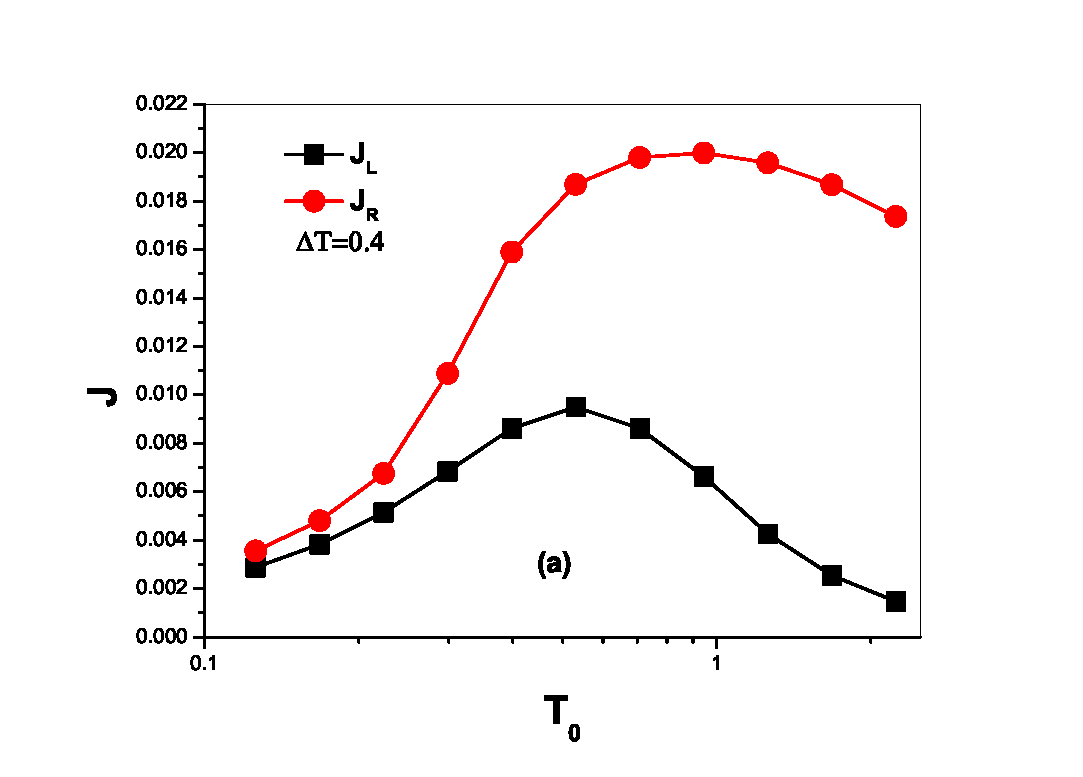
\includegraphics[width=8cm]{fig5a.eps}
\centering
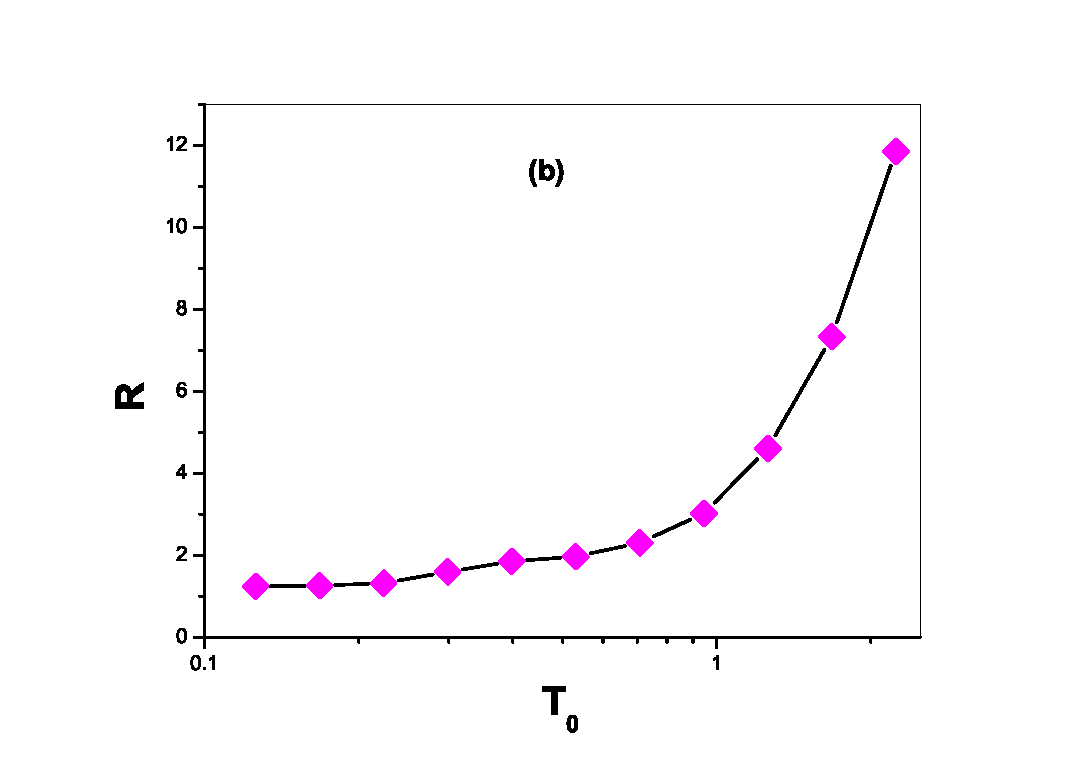
\includegraphics[width=8cm]{fig5b.eps}
\caption{(a)The heat fluxes ($J_{R},J_{L}$) as a function of the
average temperature $T_{0}=(T_{H}+T_{L})/2$. (b) the dependence of
the thermal rectification $R=\mid J_{R}/J_{L}\mid$ on the average
temperature $T_{0}$. The parameters are $\Delta T$=0.4,
$T_{H}=T_{0}(1+\Delta T)$, $T_{L}=T_{0}(1-\Delta T)$, $A=1.0$,
$K=1.0$, $M_{max}=10.0$, $M_{min}=1.0$, $N=32$.}
\end{figure}
\indent Figure 5(a) depicts the dependence of the thermal currents
($J_{R},J_{L}$) on the average temperature $T_{0}$ of chain. For a
larger $T_{0}$, both $J_{L}$ and $J_{R}$ decrease with increasing
the average temperature $T_{0}$, which is related to nonlinear
localized rotational modes of chain\cite{a27,a28}. Figure 5(b)
presents thermal rectification efficiency $R$ as a function of the
average temperature $T_{0}$. The rectification efficiency $R$
monotonically increases as the average temperature $T_{0}$
increases. It might be inferred: more phonons would be generated
with rising the average temperature $T_{0}$. Large mounts of phonons
of low-frequency collides and would be converted to phonons of
high-frequency, which increases the weight of phonons of
high-frequency and reduces the weight of phonons of low-frequency in
entire phonons spectrum.\\
\begin{figure}
\centering
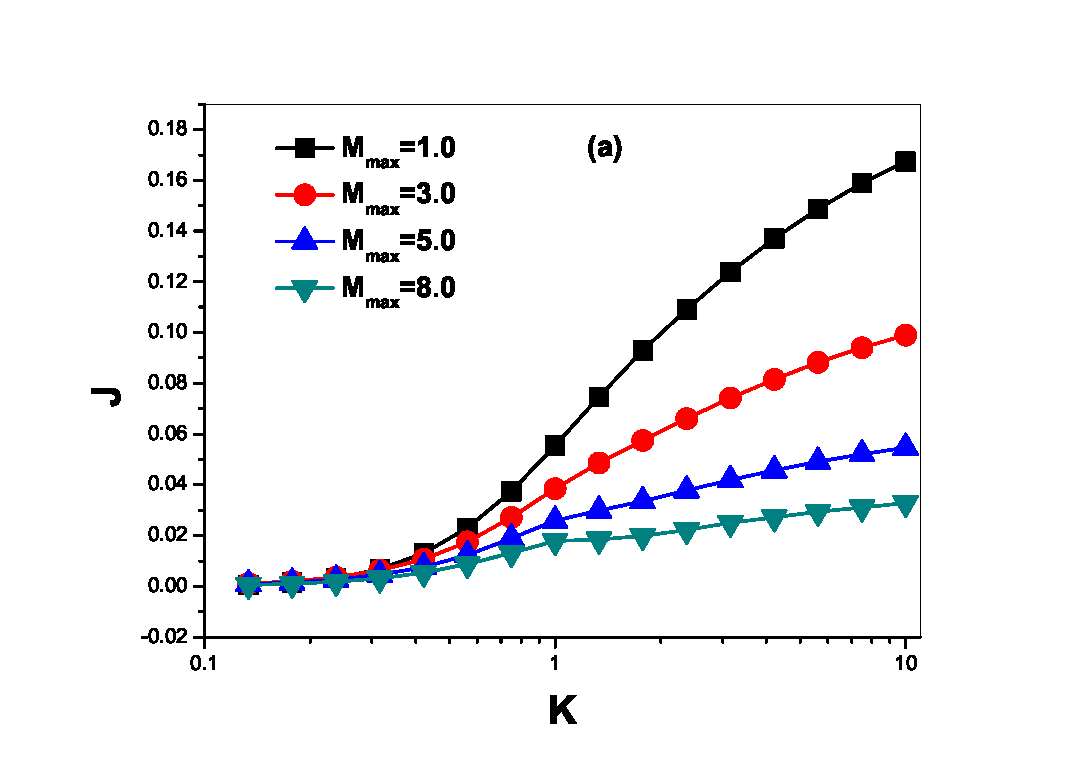
\includegraphics[width=8cm]{fig6a.eps}
\centering
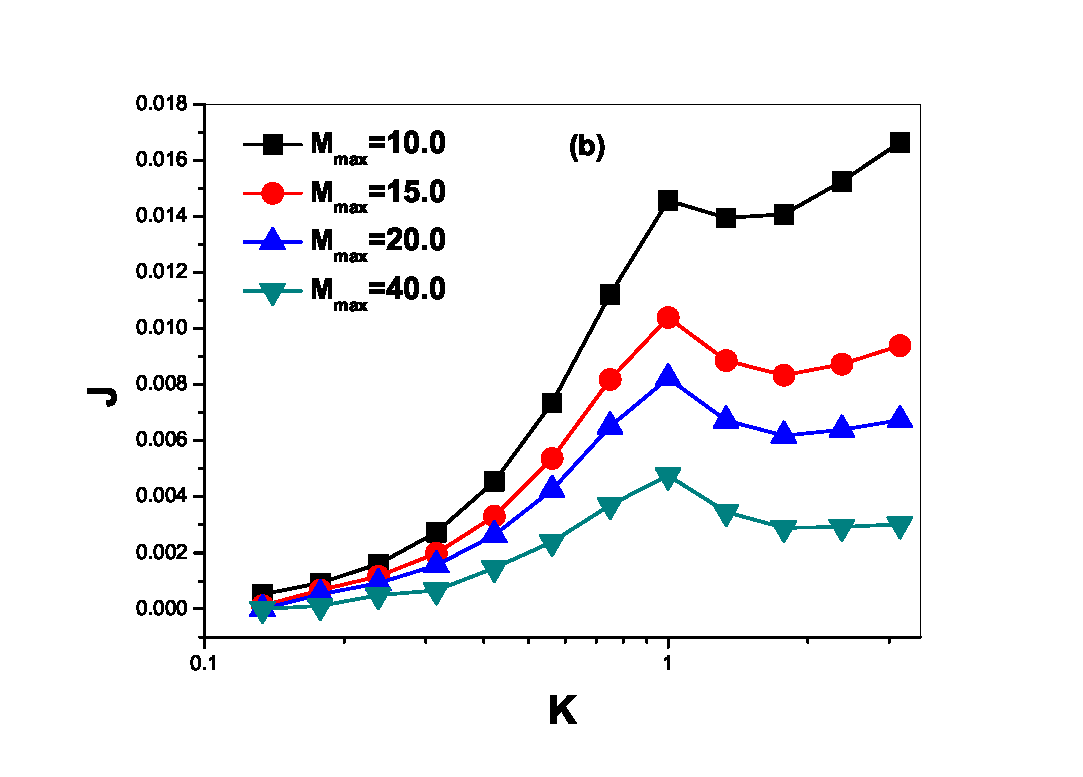
\includegraphics[width=8cm]{fig6b.eps}
\caption{The heat fluxes $J$ as a function of the strength $K$ of
the nearest-neighbor interaction for different values of the
heaviest mass. (a) $M_{max}$=1.0, 3.0, 5.0 and 8.0. (b)
$M_{max}$=10.0, 15.0, 20.0 and 40.0. The parameters are $A=1.0$,
$T_{L}=0.1$, $T_{H}=0.5$, $M_{min}=1.0$, $N=32$.}
\end{figure}

\indent In order to investigate the effects of the mass gradient on
the phenomenon that $J_{R}$ decreases with increasing the strength
$K$ of nearest-neighbor interactions, we obtained Figure 6(a) and
Figure 6(b) by nonequilibrium molecular dynamics simulations(NEMD).
Figure 6 shows the dependence of $J_{R}$ on the strength $K$ of
nearest-neighbor interactions for various values of mass gradient.
When the mass gradient is small $(e.g. \Delta M<5.0)$, the
phenomenon that $J_{R}$ decreases with $K$ increasing does not
occur. However, in case of$(e.g. \Delta M>5.0)$, that phenomenon
emerges and the maximum value of the average thermal current is
gained at $K=1.0$ for different mass gradients. It might be regarded
as the result of the competition of the increment of thermal
conductance originating from increasing $K$\cite{a23} and the
decrement of thermal conductance resulting from the existence of
localized gradons modes\cite{a31} caused by mass gradient. In case
of $\Delta M<5$, the rising thermal conductance induced by increment
of $K$ dominates the system. However,
for increasing $\Delta M$, localized gradons modes\cite{a31} is such non-ignorable that leads to the decrement of the thermal currents. \\
\begin{figure}
\centering
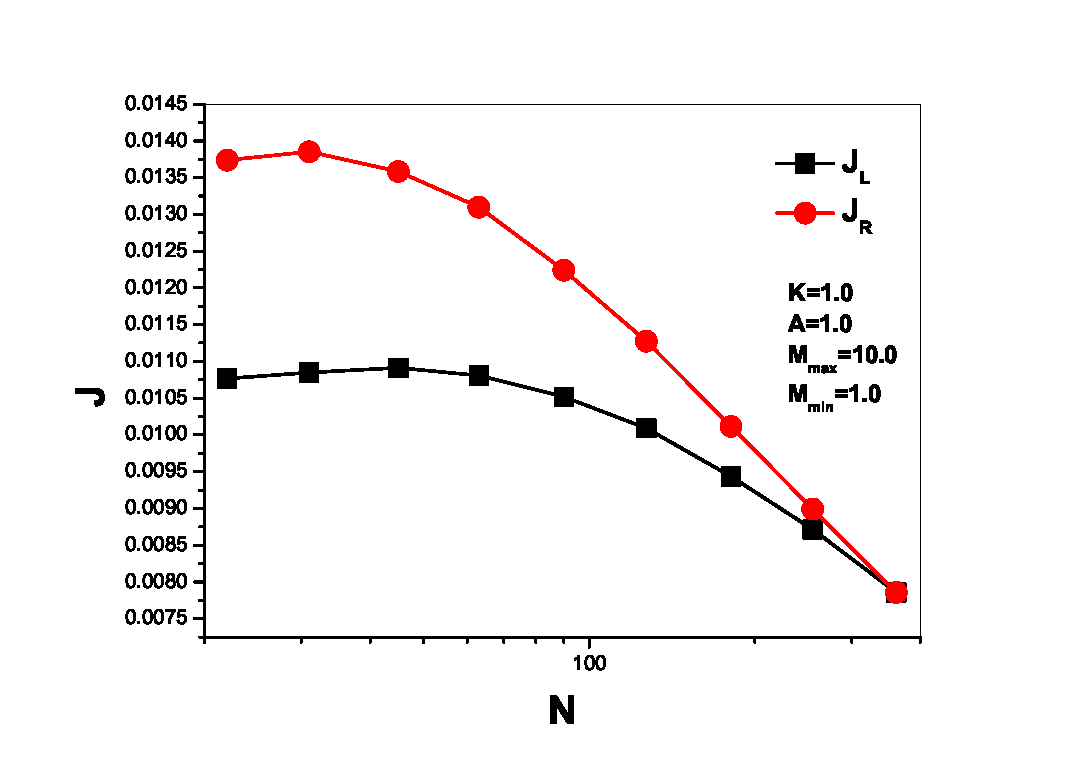
\includegraphics[width=8cm]{fig7a.eps}
\centering
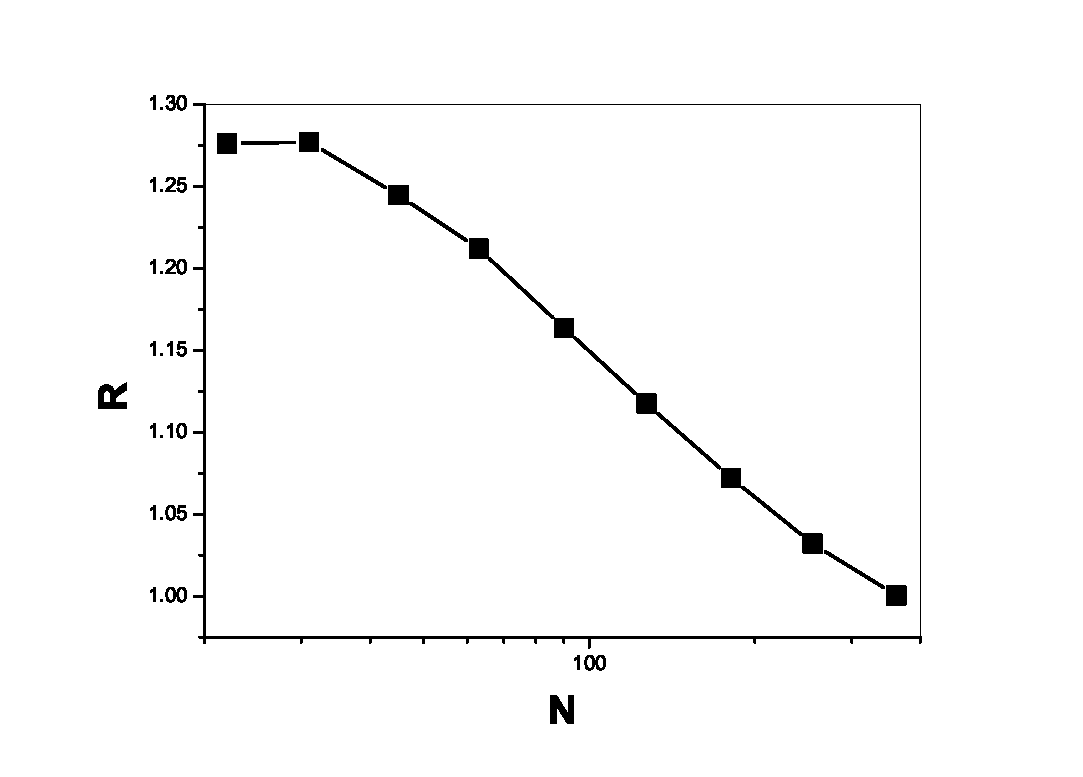
\includegraphics[width=8cm]{fig7b.eps}
\caption{(a)The heat fluxes ($J_{R},J_{L}$) as a function of the total
particles number $N$. (b) the dependence of the thermal
rectification efficiency $R$ on the system size $N$. The parameters
are $A=10.0$, $K=1.0$, $M_{max}=10.0$, $M_{min}=1.0$, $T_{L}=0.1$,
$T_{H}=0.5$.}
\end{figure}

\indent Figure 7(a) depicts the average thermal currents
($J_{R},J_{L}$) as a function of the system size $N$ for $K=1.0$,
$A=1.0$, $M_{max}=10.0$, $M_{min}=1.0$, $T_{H}=0.5$, $T_{L}=0.1$. It
is found that the heat fluxes $J_{R}/J_{L}$ all decrease if the
system size increases. Obviously, the difference of amplitude of
$J_{L}$ and $J_{R}$ gradually becomes
  smaller and smaller, which indicates thermal rectification effect gradually vanishes at a larger system size.\\
\indent According to above investigations on how the shape
parameters influence the thermal rectification efficiency, the
optimum parameters are selected to construct the thermal rectifier,
whose rectification efficiency has reached
$R=70$ (see Fig. 8).\\
\begin{figure}
\centering
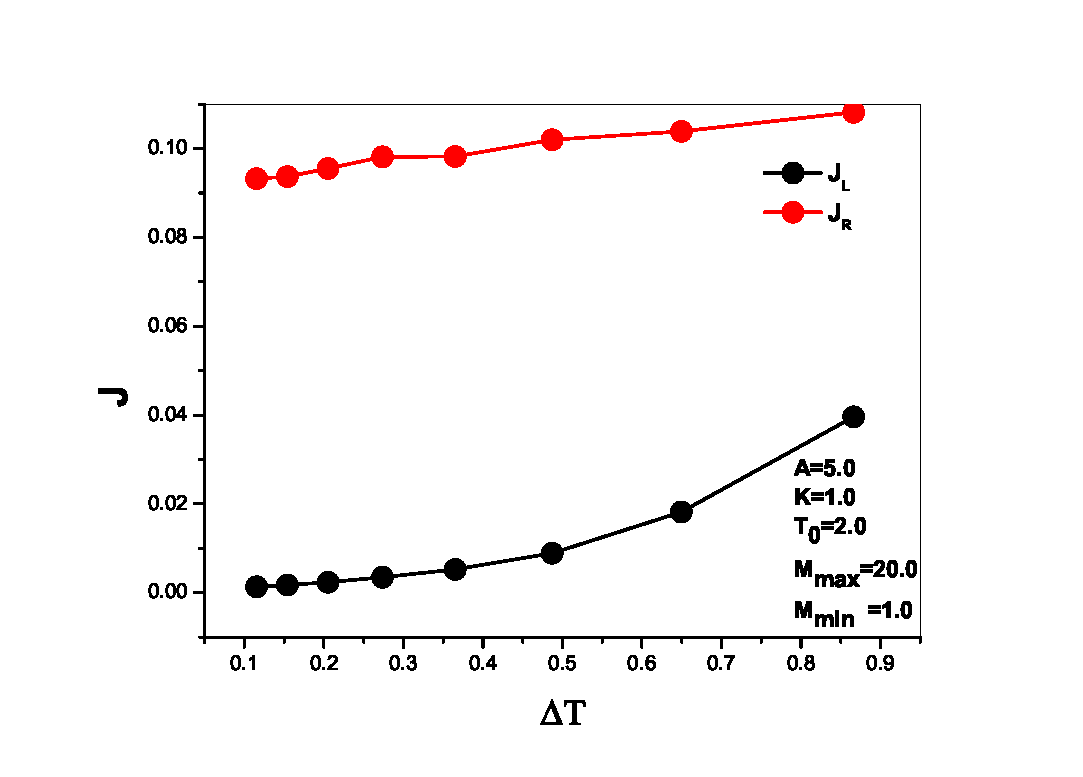
\includegraphics[width=8cm]{fig8.eps}
\caption{The heat fluxes ($J_{R},J_{L}$) as a function of $\Delta T$
with $T_{L}$ being fixed. The parameters are $A=10.0$, $K=1.0$,
$M_{max}=20.0$, $M_{min}=1.0$, $T_{L}=0.1$, $N=32$.}
\end{figure}
\section{Concluding Remarks}
\indent Heat conduction in the coupled rotator model with mass
gradient has been investigation. Using nonequilibrium molecular
dynamic simulation, the thermal currents through graded mass coupled
rotator chain largely differ when
 the heat baths are reversed, which shows the thermal rectification effect.  As for
the coupled rotator model with graded mass, it is firstly found
  that the heat flux $J_{R}$ in the direction of mass increasing is much larger than the
 heat current $J_{L}$ in the direction of mass decreasing, which is opposite to that of the one-dimensional (1D) FPU lattices with graded mass\cite{a19}. It might be explained by match/mismatch of
 the frequency spectra. By further investigation, the larger is the mass gradient $\Delta M$,
 the more evident is the thermal rectification effect, which is in accordance with the graded mass FPU-$\beta$ lattices\cite{a19,a20}.
 Secondly, the shape parameter $A$ and $K$ of nearest-neighbor interaction have influences on the thermal
 rectification. However, the phenomenon that the heat flux $J_{R}$ decreases with $K$ increasing is
 surprised. The reason is that the competition of the increasing
 thermal conductance arisen from the increment of $K$ and localized
 gradons modes induced by uniform mass distribution. Thirdly, It is found that
 the thermal rectification efficiency becomes larger with increasing the average temperature. Due to increment of the average temperature, the proportion of high-frequency phonons in entire
 phonons spectrum enhances. It leads to enhancement of the degree of mismatch of frequency spectrum at the two ends of
 atomic chain. Finally, based on above investigations, a relative optimum
thermal rectifier has been constructed and its thermal
rectification efficiency $R=\mid J_{R}/J_{L}\mid=70$.\\

\begin{thebibliography}{}
\bibitem{a1}S. Lepri, R. Livi, and A. Politi, Phys,Rep.371, 1
(2003); A, Dhar, Adv. Phys. 57, 457 (2008).
\bibitem{a2}N. Li, J. Ren, L. Wang, G. Zhang, P. Hanggi, and B. W.
Li, Rev. Mod. Phys. 84, 1045 (2012).
\bibitem{a3}B. W. Li, L wang, and G. Casati, Appl. Phys.
lett. 88  (2006) 143501.
\bibitem{a4}L. Wang, and B. W. Li, Phys. Rev. Lett. 101 (2008)
267203.
\bibitem{a5}L. Wang, and B. W. Li, Phys. Rev. Lett. 99 (2007)
177208.
\bibitem{a6}J. P. Wu, L. Wang, and B. W. Li, Phys. Rev. E 85
(2012) 061112.
\bibitem{a7}C. W. Chang, D. Okawa, A. Majumda, and A. Zettl, science
314, 1121(2006).
\bibitem{a8}M. Terraneo, M. Peyrard, and G. Casati, Phys. Rev. Lett. 88,
094302 (2002).
\bibitem{a9}B. W. Li, L. Wang, and G. Casati, Phys. Rev.
Lett. 93 (2004) 184301.
\bibitem{a10}B. Li, J. H. Lan, and L. wang, Phys. Rev. Lett. 95, (2005)
104302.
\bibitem{a11}W. Kobayashi, Y. Teraoka, and I. Tereasaki, Appl. Phys. Lett.
95, (2009) 171905.
\bibitem{a12}B. Hu, and L. Yang, chaos. 15, (2005) 015119.
\bibitem{a13}J. Lan, and B. Li, Phys. Rev. B. 74, (2006) 214305.
\bibitem{a14}J. Lan and B. Li, Phys. Rev. B. 74, (2007) 214302.
\bibitem{a15}T. S. Komatsu and N. Ito, Phys. Rev. E. 81, (2010) 010103.
\bibitem{a16}G. Casati, C. Mejia-Monasterio, and T. Prosen, Phys. Rev.
Lett. 98, (2007) 104302.
\bibitem{a17}C. R. Otey, W. T. Lau, and S. H. Fan, Phys. Rev. Lett. 104, (2010)
154301.
\bibitem{a18}M. R. Bastida, and J. M. Arizmendi-Carvajal, J. Phys. A: Math. Theor. 46, (2013)
115006.
\bibitem{a19}N. Yang, N. Li, L. Wang, and B. Li, Phys. Rev. B 76, (2007)
020301(R) .
\bibitem{a20}Tejal N. Shah and P.N. Gajjar, Phys. Lett. A. 376, (2012)
438-441.
\bibitem{a21}T. Hu, K. Hu, and Y. Tang, physica. B. 405, (2010)
4407-4412.

\bibitem{a22}Emmanuel Pereira, Phys. Rev. E 82 (2010) 040101.
\bibitem{a23}B. Q. Ai, W. R. Zhong, B. Hu, J. Phys. Chem. C 116, 13810 (2012); B. Q. Ai and B. Hu, Phys. Rev. E 83, 011131 (2011); B. Q. Ai, W. R. Zhong, B. Hu, Phys. Rev. E 83, 052102 (2011).
\bibitem{a24}Z. Nan, and J. S. Wang, Phys. Rev. B. 78 (2008) 024305.
\bibitem{a25}W. R. Zhong, W. T. Huang, X. R. Dong, B. Q. Ai, Appl. Phys. Lett. 99, 193104(2011); W. R. Zhong, M. P. Zhang, B. Q. Ai, D. Q. Zhen, Appl. Phys. Lett. 98, 113107 (2011).
\bibitem{a26}R. L. Honeycutt, Phys. Rev. A 45 (1992) 600.
\bibitem{a27}O. V. Gendelman, Phys. Rev. Lett 84 (2000) 2381.
\bibitem{a28}C. Giardina, R. Livi, A. Politi, and M. Vassalli, Phys. Rev. Lett 84 (2000) 2144.
\bibitem{a31}J. J. Xiao, K. Yakubo, and K. W. Yu, Phys. Rev. B. 73
(2006) 054201.
\end{thebibliography}
\end{document}
